\section{Defects}

\index{defects}
\begin{figure}
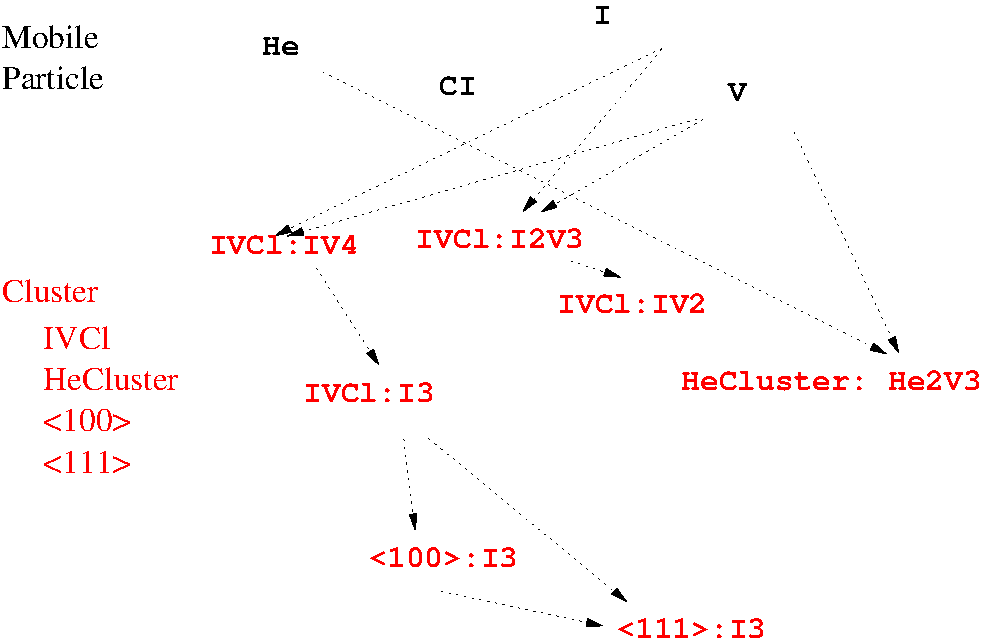
\includegraphics[width=12cm]{images/defect-evolution}
\caption{Different generic defects and their evolution}
\label{fig:defects-evolution}
\end{figure}

Figure~\ref{fig:defects-evolution} shows the generic defect evolution for OKMC simulations in  \MMonCa{}. It starts from point defects, either intrinsic, like interstitials or vacancies, or extrinsic as impurities or dopants. This defects can react between them producing other defective objects. This objects are:
\begin{description}
\item[MobileParticle]\index{MobileParticle} A single particle (point) defect. Migration, \idx{break-up} and FT emission are possible. 
\item[Cluster]\index{Cluster} Anything that is not a mobile particle. It can be extended defects ($I_8$), clusters ($He_4V_5$), combinations ($I_8CP_3$), amorphous pocktes ($I_8V_4$) etc. They can migrate, transform from to other Clusters, trap and re-emit mobile particles, recombine IV pairs and trap other multiclusters. They can have particular shapes. 
\item[Interfaces] \idx{Interfaces} are not formed by particles, although they can contain particles. They are 2D surfaces that separate different materials. They can trap, emit and annihilate particles, and can annihilate clusters. Particle diffusion on the interfaces is also possible.
\end{description}

\section{Definition of defects}
\index{defects!definition}\index{definitions}

The defects being used in the simulation are defined in the \param{Models} file for each material. Description of the important definitions there follow.

\subsection{particles}

Defines the \param{particles} to be used in the material. For instance:
\begin{lstlisting}
map<string,bool> particles { 
	HeI true 
	He  true
	HeV true
	I   true
	V   true
	C   true
	CI  true
	CV  true
}
\end{lstlisting}

\subsection{defined}
\index{defined}
Defines wich generic defects will be used (true/false). There are no reserved words. Any name will be understood as an implemented cluster. For instance, \param{ICluster}, \param{Void}, \param{BICs}, \param{IVCluster}, etc.

An example is
\begin{lstlisting}
map<string,bool> defined { 
	IVCluster true 
	ICluster  true
	VCluster  true
	BICs      true
}
\end{lstlisting}

\subsection{interactions}
\index{interactions}

The parameter \param{interactions} is used to:
\begin{itemize}
\item \index{interaction} Specify whether the interaction between particular defects is allowed or disabled. 
\item \index{capture radius} Specify, optionally, the capture radius for a particular interaction. The interaction will happen when the distance between two particles belonging to each defect is smaller or equal than the specified capture radius. If not specified, the default value of \param{lambda} is used.
\end{itemize}

This parameter requires a list of all possible interactions. Wildcards are allowed for interactions involving \param{Clusters}. The result of interactions allow an optional capture radius for the particular interaction listed. All interactions have the following format:
\begin{lstlisting}
Reactant1+Reactant2  0/true/false/result[,probability][,capture radius]
\end{lstlisting}

The logic for the \idx{reaction syntax} is the following:
\begin{itemize}
\item Reactions between mobile particles giving a particle are defined con true/false.
\item Reactions between clusters, are defined with true/false.
\item Reactions between particles, producing a cluster, are defined with the name of the cluster and the probability to follow that path.
\item In the particular case of reactions between mobile particles producing a recombination, 0 can be specified indicating instant recombination.
\item Reaction between a defect and an interface are specified with true/false.
\item For reactions between particles, particles and clusters, or clusters (i.e., all except interfaces) an optional \idx{capture radius} can be specified.
\end{itemize}

Reactants are the inputs for the \idx{interaction}s.  

The procedure to define interactions, assuming that M is the name of a unary material, is defined in Table~\ref{tab:interactions}.

\begin{sidewaystable}
\caption{Reactions defined in Models/interactions. M represents the material for binary materials, being empty for unary ones. A represents an ``impurity'', an element not constituting the material.}
\label{tab:interactions}
\begin{tabular}{|l|ccl|c||l|}
\hline

Generic &Reactant 1 & Reactant 2 &result& example & comments\\\hline
\hline
MP+MP & MI       & MV       & 0 or MC,prob     & MI+VM IVCluster,1   & 0 means annihilation\\\hline
MP+MP & MI       & MI       & MC,probability   & MI+MI ICluster,0.4  & Total probability should be 1.\\\hline
MP+MP & MV       & MV       & MC, probability  & MV+VM VCluster,1    & Similar to I+I\\\hline
MP+MP & MI or MV & AM       & true             & MI+CM true          & Produces another MP\\\hline
MP+MP & MI       & AV       & true             & MI+HeV true         & Produces another MP\\\hline
MP+MP & MV       & AI       & true             & MV+HeI true,0.3     & A capture radius is specified\\\hline
MP+MP & MI or MV & AI or AV & MC,probability   & MV+CV CCluster,1    & Produces a MC\\\hline
MP+MP & AM       & AI or AV & MC,probability   & CM+CV CCluster,.5   & Produces a MC\\\hline
MP+MP & AV or AI & AV or AI & MC,probability   & HeV+HeV HeCluster,1 & Produces a MC\\\hline
\hline

MC+MP & MC:ID & MP& true/false & HeCluster:He2V2+mI  true     & \specialcell{Wildacards allowed,\\as in HeCluster:*+mI true}. \\\hline
MC+MC & MC    & MC& true/false & HeCluster+HeCluster true,0.5 & \specialcell{All or nothing, with\\a non-standard capture radius}.\\\hline
\hline

MP+Int & MP & Material & true/false & mI+Gas true        & \specialcell{Reactions with an interface\\with the specified material}. \\\hline
MC+Int & MC & Material & true/false & HeCluster+Gas true & \specialcell{Cluster reaction with specified material}.\\\hline
\end{tabular}
\end{sidewaystable}

All the possible interactions, and their capture radius, that can be defined are summed up in Table~\ref{tab:possibleinteractions}. If a \idx{capture radius} is not specified it is taken as the default value of \param{lambda} for the material.

\begin{table}
\caption{Results of the defined interactions}
\label{tab:possibleinteractions}
\begin{center}
\begin{tabular}{|c||c|c|}
\hline
            & \textbf{MP}              & \textbf{MC}  \\\hline\hline
\textbf{MP} & \specialcell{MP MC\\ 0 } & MC           \\\hline
\textbf{MC} & MC                       & MC           \\\hline
\end{tabular}
\end{center}
\end{table}

The interactions are:

\begin{itemize}
\item Mobile particles interact with mobile particles.
\item If a Cluster is formed, the multicluster name and the probability is written (i.e., $<$111$>$,1).
\item If there is a recombination, either 0 or Cluster is written.
\item For MobileParticles, true is written.
\item For interfaces, the interface is written as second reactant: e.g. MI+Gas, $<$111$>$+Gas. They interact with everything.
\end{itemize}

